\section{Background}


	- Allgemeine Vorstellung der Packages ihr Vor und Nachteile
	
	\subsection{GetOldTweets3-Pakage}
	%\begin{justify}
	
	GetOldTweets3 ist ein kostenlose Python 3 Packages mit welchen Twitterdaten ohne API-Schlüssel abgerufen werden können.
	Mit GetOldTweets3 können Sie Tweets mit einer Vielzahl von Suchparametern wie Start-/Enddatum, Benutzername(n), Textabfrage 
	und Referenzortbereich durchsuchen. Außerdem können Sie angeben, welche Tweet-Attribute Sie einbeziehen möchten. Einige Attribute
	sind: Nutzername, Tweettext, Datum, Retweets und Hashtags.\citeint{userguid} 
	Die offizielle API von Twitter hat eine lästige Zeiteinschränkung, weshalb man keine Tweets älter als eine Woche abrufen 
	kann. Es gibt einige Tools die Zugang zu älteren Tweets anbieten, diese sind jedoch meistens kostenpflichtig. Das Forscher-
	team hat nach einem andere Tool gesucht die diese Aufgaben übernehmen, wodurch die Wahl auf das Package GetOldTweets3 gefallen 
	ist.\citeint{python}   	
	Die Analyse des Codes von GetOldTweets3 und die Funktionsweise des Searchthrough Browsers von Twitter zeigt wie das Packages auch
	an alte Tweets kommt. Grundsätzlich, wenn sie auf Twitter seiten eingeben oder User suchen, startet ein Scroll-Loader. D.h. wenn sie
	dann weiter nach unten scrollen, bekommen sie immer mehr Tweets zu den Suchbegriffen. Diese ganzen Tweets bekommen sie durch Abfragen 
	an einen JSON-Provider. GetOldTweets3 imitiert den Searchthrough Browser von Twitter um den Scroll-Loader zu starten und zieht sich dann 
	anhand, der Abfragen an einen JSON-Provider die JSON-Datei und gibt diese decodiert zurück um dann alle Twitts anhand der oben gegebenen 
	Parameter herauszufiltern. Dies kann man in Quelle \citeint{github}, dem Github-Repositorium gut nachvollziehen. Somit ist es möglich sowohl 
	aktuelle als auch sehr alte Tweets zu scrapen.\citeint{github}
	
	
	\begin{figure}[ht]
		\centering
		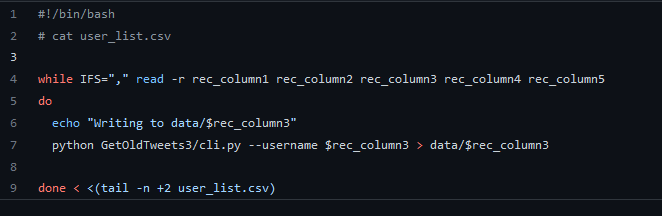
\includegraphics[width=0.9\textwidth]{images/Kapitel2/Code_Beispiel_1}
			\caption{\label{fig:CodeBeispiel}Code Beispiel für das Scrapen der Tweets}{Ist eine Python Bibliothek mit der Twitter Daten durch den Scroll-Loader 
			        des Searchthrough Browsers von Twitter als JSON-Datei abgerufen werden können.}
	\end{figure}
	
	
	So kann durch eine paar Zeilen Code, wie man in der Abbildung \label{polPolar} sieht, eine bash-Datei erstellt werden, durch welche die Daten gesucht und 
	abgespeichert werden. Das Scraping an sich kann durch die Größe der JSON-Datei einige Zeit in Anspruch nehmen. Wir haben gerade mal 2 Millionen Tweets 
	insgesamt bei einer Laufzeit von ca. 35 Stunden.  
	
	%\end{justify}

	\subsection{NLTK-Natural language Toolkit}
	%\begin{Absatz}
	- Vllt Klären warum wir nicht NLTK verwendet haben, sondern Textblob
	- Vorteile von Textblob gegenüber NLTK
	- Nachteile von Nltk	
	
	%\end{Absatz}

	\subsection{TextBlob}
	%\begin{Absatz}
	- Textblob: Vllt. herausfinden wie die Berechnung stattgefunden hat	
	- Vorteile von Textblob gegenüber NLTK
	- Warum haben wir das Tool genutzt.	
	
	%\end{Absatz}

	\subsection{Sparks}
	%\begin{Absatz}
	- Aus der Vorlesung Vorteile von Spark finden und einbauen	
	
	%\end{Absatz}


	
